\documentclass[letterpaper,12pt]{article}   %%% Can be report

%% set paper margins
\oddsidemargin=0.1in
\evensidemargin=0.1in
\textwidth=6.0in
\topmargin=-0.7in
\textheight=9.0in
\parindent=0.2in

\usepackage{amsmath,amssymb,bm}
\usepackage{graphicx}
\usepackage{rotating}
\usepackage{float}
\usepackage{subfigure}
\graphicspath{%
  {figs/ipe/}
  {figs/dia/}
  {figs/matlab/}
  {figs/imag/}
} 
\usepackage[width=11cm,font=footnotesize,labelfont=bf, %
format=default,justification=centerlast]{caption} % Figure caption text customization 

\usepackage{pgfgantt}


\usepackage{hyperref}
\usepackage{soul}
\usepackage{setspace}
\usepackage{multirow}

\usepackage{siunitx}
\sisetup{unitsep=\cdot}

\title{ECE498:~Senior Capstone Project I\\\textbf{\underline{Project Proposal}}\\
\vspace{0.5in}
Project Title: Development of an Intelligent Building Energy Management Platform}
\vspace{1.5in}
\author{Brian Lauer and Elliot Watkins\\ Advisor: Dr.~Suruz Miah
}
%\date{February 6, 2003}  No need to write, Date will be automatically on the title page
\date{}  % Do not show date on the title page

%%%%%%%%%%%%%%%%% Set document line spacing %%%%%%%%%%%%%%%%%%%%%
\singlespacing
%\onehalfspacing
%\doublespacing
% all packages are in the following tex file.
%\input{paper-preamble.tex}
\begin{document}

%%% Make title page 
\begin{titlepage}
 \maketitle

\vspace*{4.0cm}
\begin{center}
\normalsize
Electrical and Computer Engineering Department\\
Caterpillar College of Engineering and Technology\\
\href{http://www.bradley.edu/}{Bradley University}\\

\vspace*{6.0cm}
\copyright~B.~Lauer~and~E.~Watkins, Peoria, IL, USA, 2020\\

\end{center}
\thispagestyle{empty}

\end{titlepage} 
%%%%%%%%%%%%
%\thispagestyle{empty}
%\maketitle
\newpage
\renewcommand{\contentsname}{Table of Contents}
\tableofcontents
\newpage

\section{Introduction} %introduction (basically what was in the abstract before)
The Internet of Things is a large network of embedded devices like sensors, wearables, and appliances capable of receiving control commands and reporting data over the Internet. Many industries take advantage of this infrastructure to improve process flow and efficiency. One of these industries is the commercial and industrial sector which often employ building automation or management systems to help better manage processes or devices in a building like air conditioning systems, lights or industrial machines. Technological advancements have allowed devices to become connected to a building network through communication protocols like WiFi, Ethernet, Modbus, or BACnet which enables them to be more easily controlled from a central system. Even further, an intelligent BEMS is able to perform further actions other than simply responding to requests from users or requesting device information through the use of machine learning algorithms to help reduce power usage in real time.

Our overall goal will be to create a platform in which users can login and access devices connected to a building's energy supply. This will allow the user to closely monitor energy usage throughout a commercial or residential building. Additionally, the user will be able to control devices connected to the platform, allowing precise control over the building's energy use.
\begin{figure}[H]
    \centering
    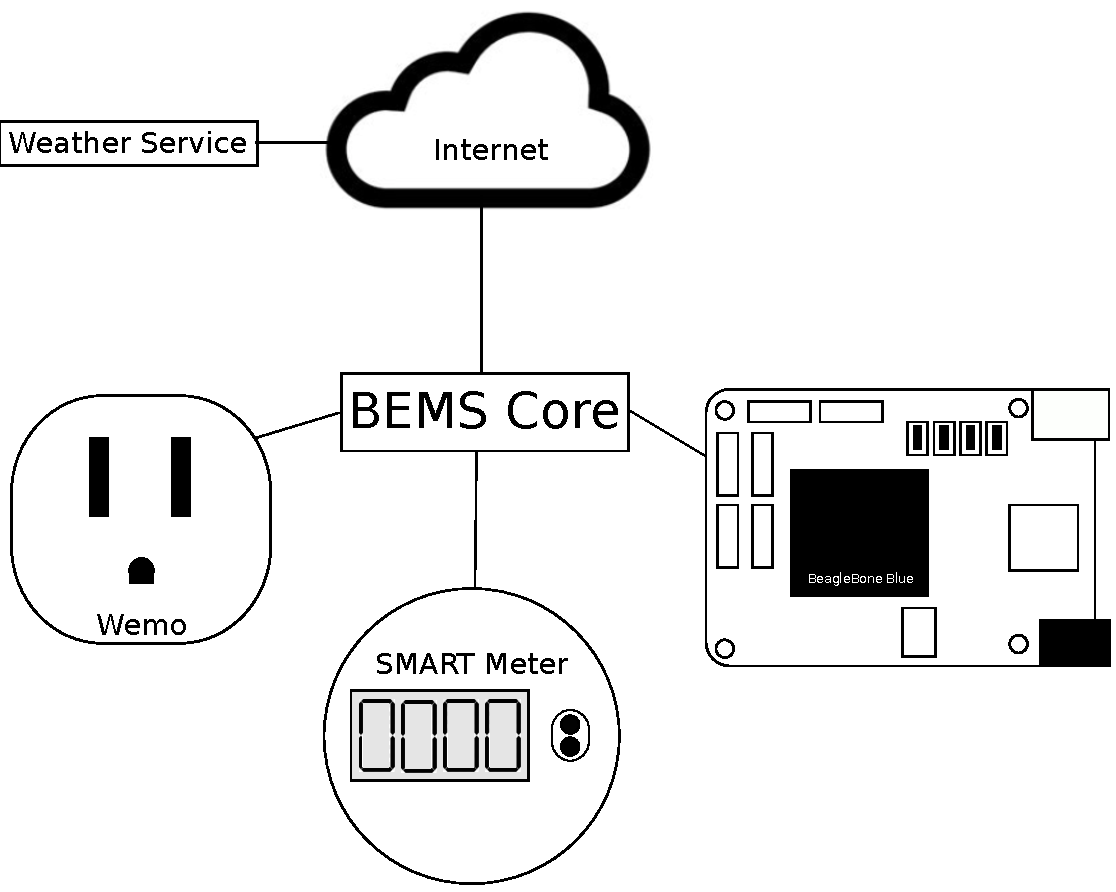
\includegraphics[scale=0.35]{figs/highLevelArchitecture.pdf}
    \caption{High Level Architecture of the Proposed System}
    \label{fig:highLevelArchitecture}
\end{figure}

The BEMS Core will interface with as many devices as it has support for. By the end of this semester, we plan to have support for the Wemo Insight Switch and the BeagleBone Blue. The user will be able to control these devices directly from the web server. Additionally, we will try to simulate a microgrid with MATLAB Simscape. Another feature we would like to add (if time allows) is a weather notification. The BEMS core will ping an online weather service routinely and notify the user of any storms likely to cause power outage in the forecast. To simulate a building HVAC system, a Simulink model will be created, and an optimization algorithm will be used to regulate the building temperature to optimize both user comfort and energy usage. 

\newpage
\section{Background Study} %review of literature and prior work
%write more here (related works from subsystem level functional requirements?)
Our BEMS is heavily derived from an existing Building Energy Management System titled Building Energy Management Open Source Software (BEMOSS)~\cite{BEMOSS}. Additionally, others have created a variety of implementations for building energy management. After thoroughly searching for related projects, we found the following resources that we believe will expedite our goals for this project.

An existing BEMS described in~\cite{Mataloto2019} incorporates its own sensors for temperature, humidity, luminosity, air quality, and motion. The data from these sensors is then fed to the BEMS core where decisions are made for the HVAC system and lighting of a building. The sensor data is transferred to the BEMS though the IoT, like our own BEMS core. 

One of the works in the literature discusses Model Predictive Control (MPC) which is a modern process control algorithm capable of taking into account current and previous time values to improve building automation~\cite{Mayer2017}. A multilevel hierarchy is presented to split control of a building into two levels: the energy supply level and user level. Example usage of this control scheme provided are temperature control of a building and its corresponding zones and interaction with a smart grid. Studies were performed on a commercial building with the building's energy supply system and hierarchy model predictive controller implemented in Matlab.

In~\cite{8246800}, the authors describe similar functional requirements to our own BEMS Core. They periodically gather power consumption and device status data and send that data to a database. We are doing exactly what they describe using the Apache Cassandra database. The authors also use an "analytics [sic] engine to process [the data] and generate reports, graphs, and charts." Our system only generates a power consumption plot for a given day, but we are still meeting this same requirement - just on a smaller scale. The communication with devices and power consumption reports are to be accessible through a web-based application that is easy to use. Again, our implementation is simple and very intuitive for the end-user. Finally, these authors mention a user-login feature. They explain that their system would include multiple levels of accessibility based on the user privileges. Our system does not currently have a user-login feature. However, in its current state, the BEMS Core simply uses a router to access devices that are also connected to the router. Since this is a closed system, users need only protect their router with a secure password.

A control scheme in~\cite{Barchi2018} is presented to manage a photovoltaic array and battery energy storage system. Tests were conducted in a shopping mall with an electronic load to emulate the power consumption of the building. Potentially, a similar technique could be used to model the energy demand of a house in Simulink or Simscape model. Through their scheme, an intelligent BEMS is used to collect measurable data like power, voltage, and current and stored for offline analysis later. Their platform collects data every five minutes compared to the 20 second polling rate currently configured in our platform. A control algorithm was presented proving that grid energy is consumed more heavily during periods of low power demand rather than PV power.

\section{System Architecture}
Before deciding on what the inputs and outputs would be, we needed to define the functional requirements. We then figured out the exact inputs and outputs as well as the necessary composition of the BEMS core to achieve our goal.
\medbreak\noindent
The minimum viable product of this project will be to connect to a Wemo Insight Smart Plug and a BeagleBone Blue. The only functionality needed on the BeagleBone Blue will be PWM input to the motor drivers. Additionally, we will be implementing a database to track power usage on both devices. Another important feature is to collect power usage data for an entire house. To simulate power usage of an entire house, we will use MATLAB Simscape to develop a microgrid and power meter. Finally, simulink will be used to simulate an HVAC system with a self-regulating (intelligent) algorithm.

\begin{figure}[H]
    \centering
    
\includegraphics[scale=0.4]{figs/functionalBlockDiagram}
    \caption{High-level Functional Block Diagram}
    \label{fig:functionalBlockDiagram}
\end{figure}

\subsection{Inputs}
This project will include input from users, smart power meter, devices, and a weather service. Users will be able to adjust the operation of a device (turn up the temperature of an AC unit, for instance) or turn a device on or off completely. Smart power meters will be able to connect the platform and give real-time updates of the building's overall power usage. We would also like to look into meters for individual appliances like AC units and furnaces. The connected devices themselves will communicate to the web server their current status when needed. Finally, our platform will regularly receive weather updates from a weather service and warn the user about potential energy loss due to storms.

\subsection{BEMS Core}
A high level view of the operation of the software platform is shown in Figure \ref{fig:functionalBlockDiagram}. Incorporated into the platform will be a web server developed in Python with the Flask web framework. All external and internal HTTP (Hyper Text Transfer Protocol) requests will be processed through this web server in order to store device or user information in the SQLite database. An external request is defined as a request made by a user or device to, for example, update information in the database with a series of SQLite queries. Internal requests are made by other entities or processes running in parallel on the platform including software agents. Similar to BEMOSS, these agents will help to communicate with various devices supported by the platform like broadcasting a discovery service, sending control commands to devices, and regularly requesting data from devices. The platform will be developed and deployed on a Linux machine to encourage support for deployment on SBCs (Single Board Computers) like the Raspberry Pi or BeagleBone Blue to be conveniently stored in a secure location of a building or home like a server cabinet for instance.

\medbreak\noindent
The SQLite database will be designed to store device information like the device IP address, MAC address, manufacturer name, and device name. A feature will be implemented to allow for customizing the device name. For example, a WeMo Switch connected to the building or home LAN (Local Area Network) could be renamed to "Lamp" or "Light". Secondly, a feature will be added to specify the room or location of each device within the building or home. This will aid any users of the software in distinguishing devices from each other. 
\medbreak\noindent
% Talk about time series feature
Functionality will be available in the final version of the platform to store time-series data like on/off status and power data in a database using Apache Cassandra, an open-source NoSQL database management system. This offers a convenient way to log data from device readings in real time. In the future, machine learning algorithms can be used alongside this database to help optimize energy usage.
\medbreak\noindent
A further addition to the software will be added in the form of support for Simscape models, an addon for Simulink to model electromechanical systems. Matlab scripts will be associated with each of these models to collect power data from various electrical models created with Simscape. Using TCP/IP, Matlab will send data from the associated models over the network to the platform to be stored in the Cassandra database.

\subsection{Outputs}
The BEMS Core will output all data from devices, smart power meter, and weather updates to the web server. The user will then be able to peruse all available data on any smart device connected to the network.


\section{Preliminary Work}
Prior to the start of the capstone project, work had been completed on the platform based off BEMOSS~\cite{BEMOSS}. Most of the software architecture was heavily derived from the previously developed software.
% \subsection{Modelling} \label{sec:model}

% \subsection{Simulation Results} \label{sec:simresults}

\subsection{Software Agent Design} \label{sec:design}
As part of the base requirements of the design, the platform incorporates multiple agents to help facilitate communication between various parts of the software. Some of the current agents which are Python classes in the software include
\begin{itemize}
    \item Discovery agent - Traverses through available API files and uses the \texttt{findDevices} API call to locate devices on the network, later on auto discovery will be implemented to allow devices to be shown in the software whenever a new supported device joins the network
    \item Control agent - General agent for all supported devices, capable of retrieving and modifying the status of a device available on the network through API calls, supports starting up a separate thread to periodically query the device for information like ON/OFF status and power consumption 
\end{itemize}
A flow chart of the scheme the Discovery agent uses to initialize a device in the platform is shown in Figure \ref{fig:setdevicetoactive}. To ensure a new device is only stored once in the metadata database, a query is performed to ensure that only one device exists with the recently discovered device's name. Once a new table is created in the Cassandra database for the device which is unique for the specific device, the control agent is notified to start up a new thread to collect device data.
\begin{figure}[H]
    \centering
    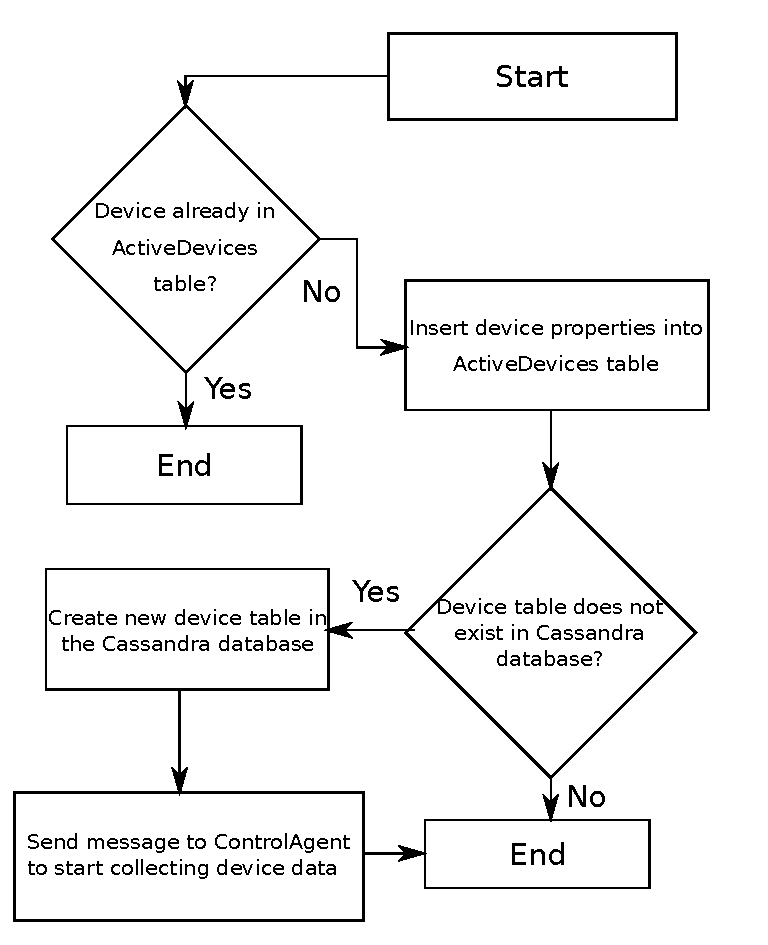
\includegraphics[scale=0.5]{figs/setDeviceToActiveFlow.pdf}
    \caption{Flow chart of the \texttt{setDeviceToActive} method}
    \label{fig:setdevicetoactive}
\end{figure}

A second algorithm that the discovery agent uses to look for devices on the network is shown in Figure \ref{fig:searchfordevices}. The process to search for available devices on the network is executed for each individual device API. Once a device has been found it is then added to the active devices table if it does not already exist.

\begin{figure}[H]
    \centering
    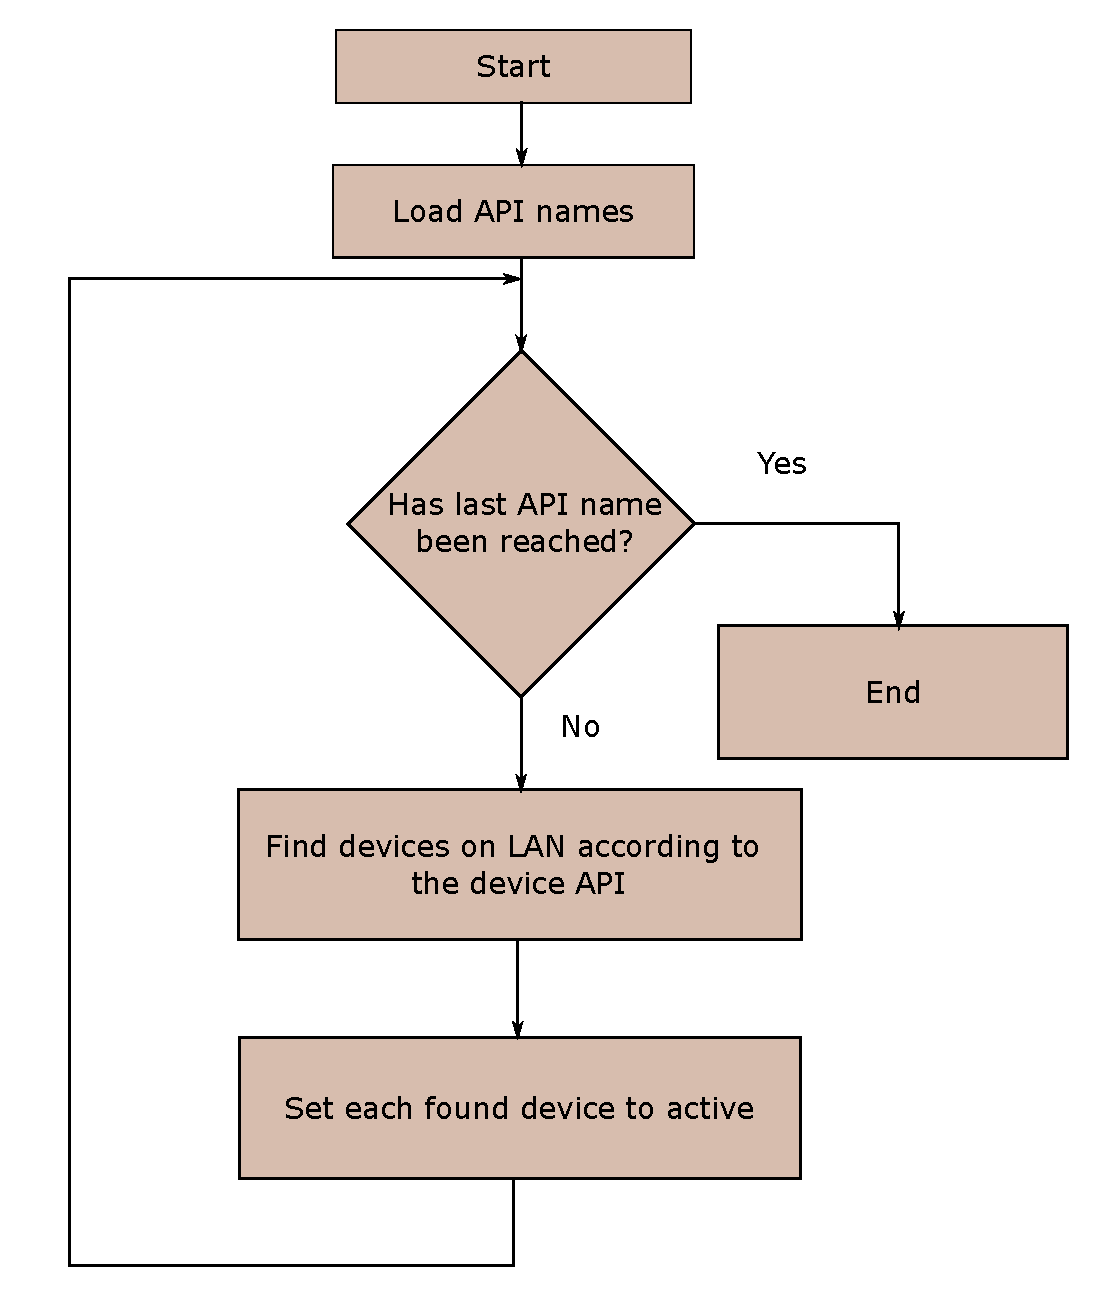
\includegraphics[scale=0.45]{figs/searchForDevicesFlow.pdf}
    \caption{Flow chart of the \texttt{searchForDevices} method}
    \label{fig:searchfordevices}
\end{figure}

\begin{figure}[H]
    \centering
    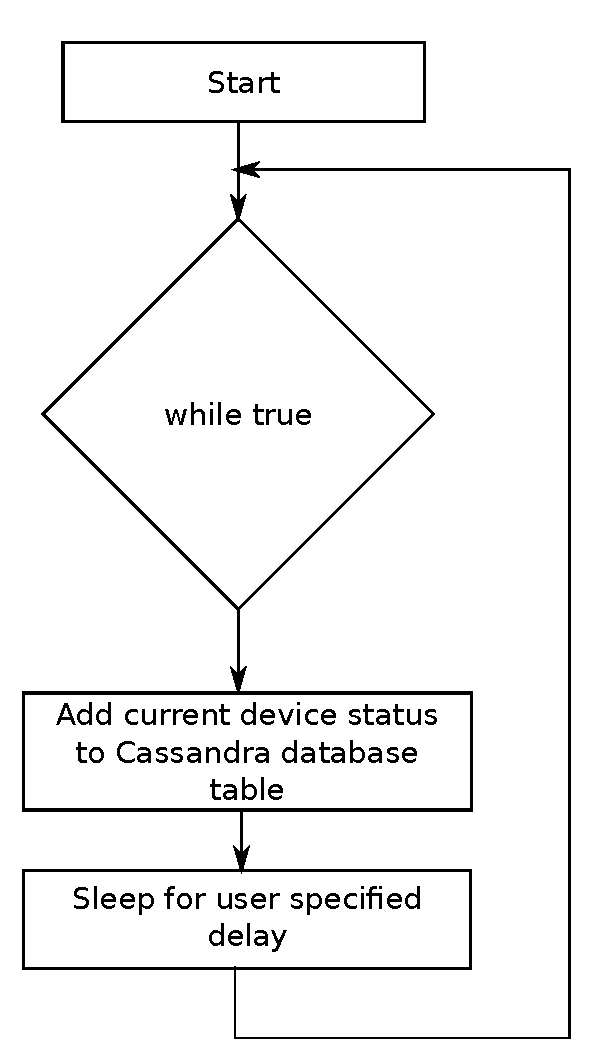
\includegraphics[scale=0.45]{figs/periodicQueryBehaviorFlow.pdf}
    \caption{\texttt{ControlAgent.periodicQueryBehavior()} flow chart}
    \label{fig:periodicQueryBehavior}
\end{figure}

More agents will likely be added later to help with supporting devices with behavior differing from that of the WeMo Switch and DC Motor. 

\subsection{Device APIs}
Common APIs are included for each supported device like \texttt{setState}, \texttt{getState}, \texttt{findDevices}, and \texttt{findMetadata}. In the WeMo Switch implementation, IP multicasting and Universal Plug and Play are utilized to send out messages to any devices listening on a multicast group with a specific IP address and port number. The location of an XML file is located whenever a Switch has been properly located on the network. This file contains information about the device including the nickname, manufacturer, and IP address as well as other information like Simple Object Access Protocol (SOAP) commands to alter the state of the device like ON/OFF status and commands to retrieve device information. The publish/subscribe model is used for communication between the web server and agents. Each agent supports a separate thread dedicated to subscribing to messages from publishers.

Support for the SQlite database has been successfully added while the Cassandra database support is still being implemented. Also, driver support is still being developed for the Beaglebone Blue and ultimately the DC motor.

\subsection{Experimental Setup} \label{sec:expsetup}
To test and validate the BEMS core, we set up a physical WeMo Insight Switch and embedded computer in the Senior Project Lab. This lab is also equipped with a router that we could use to connect to the devices. Figure 6 gives a visual explanation of our setup.

\begin{figure}[H]
    \centering
    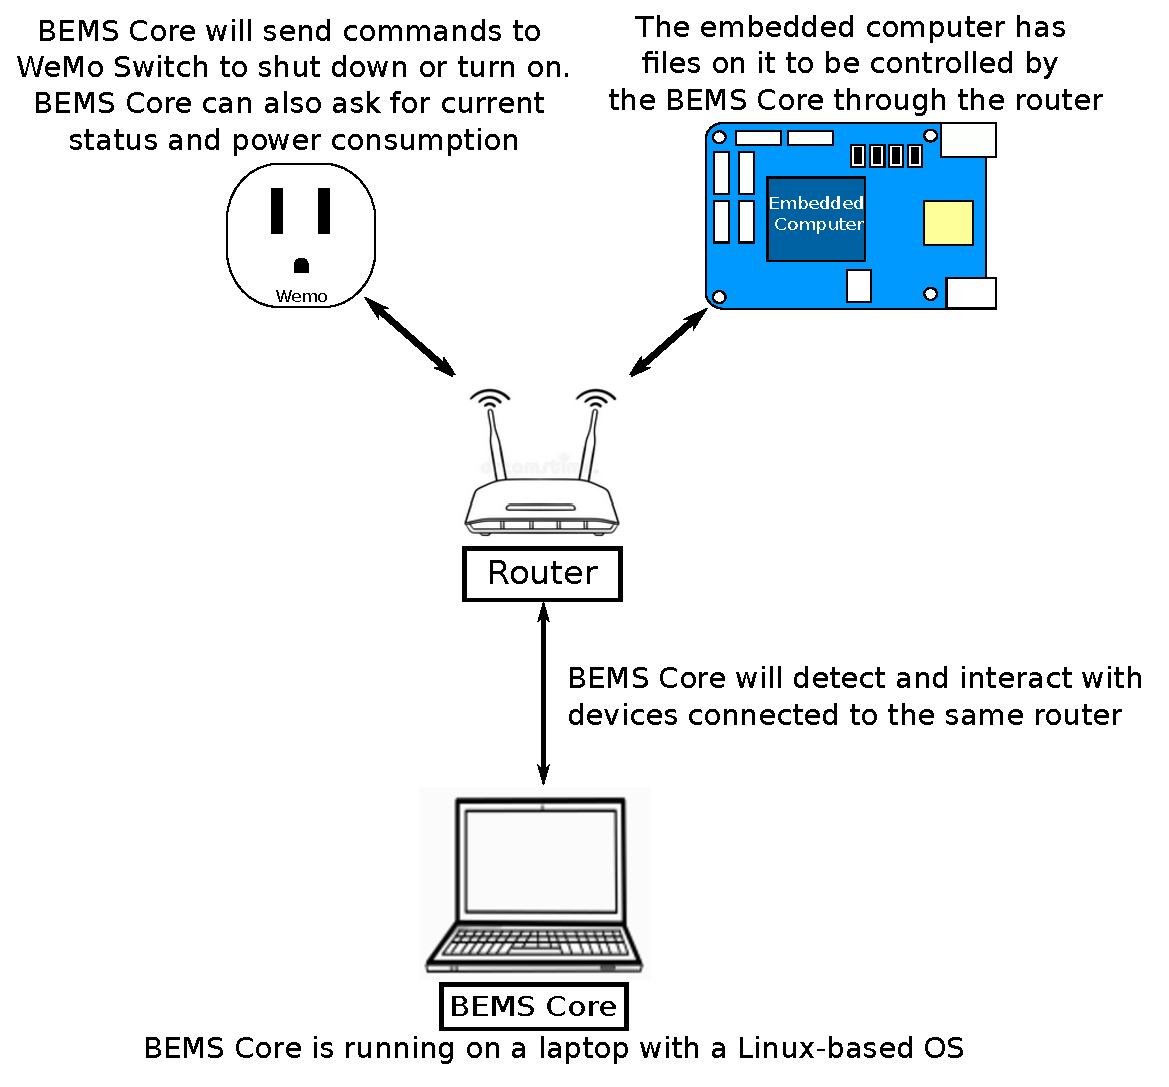
\includegraphics[scale=0.55]{figs/experimentalSetup.pdf}
    \caption{Current lab setup for testing purposes}
    \label{fig:expLabSetup}
\end{figure}

Figure 7 shows our actual setup. In the top left corner, the WeMo Insight Switch can be seen plugged into a power strip. In the lower left, we have a laptop with an Ubuntu distribution running the BEMS core. In between the 2 laptops, the embedded computer (BeagleBone Blue) is being powered by the laptop on the right.

\begin{figure}[H]
    \centering
    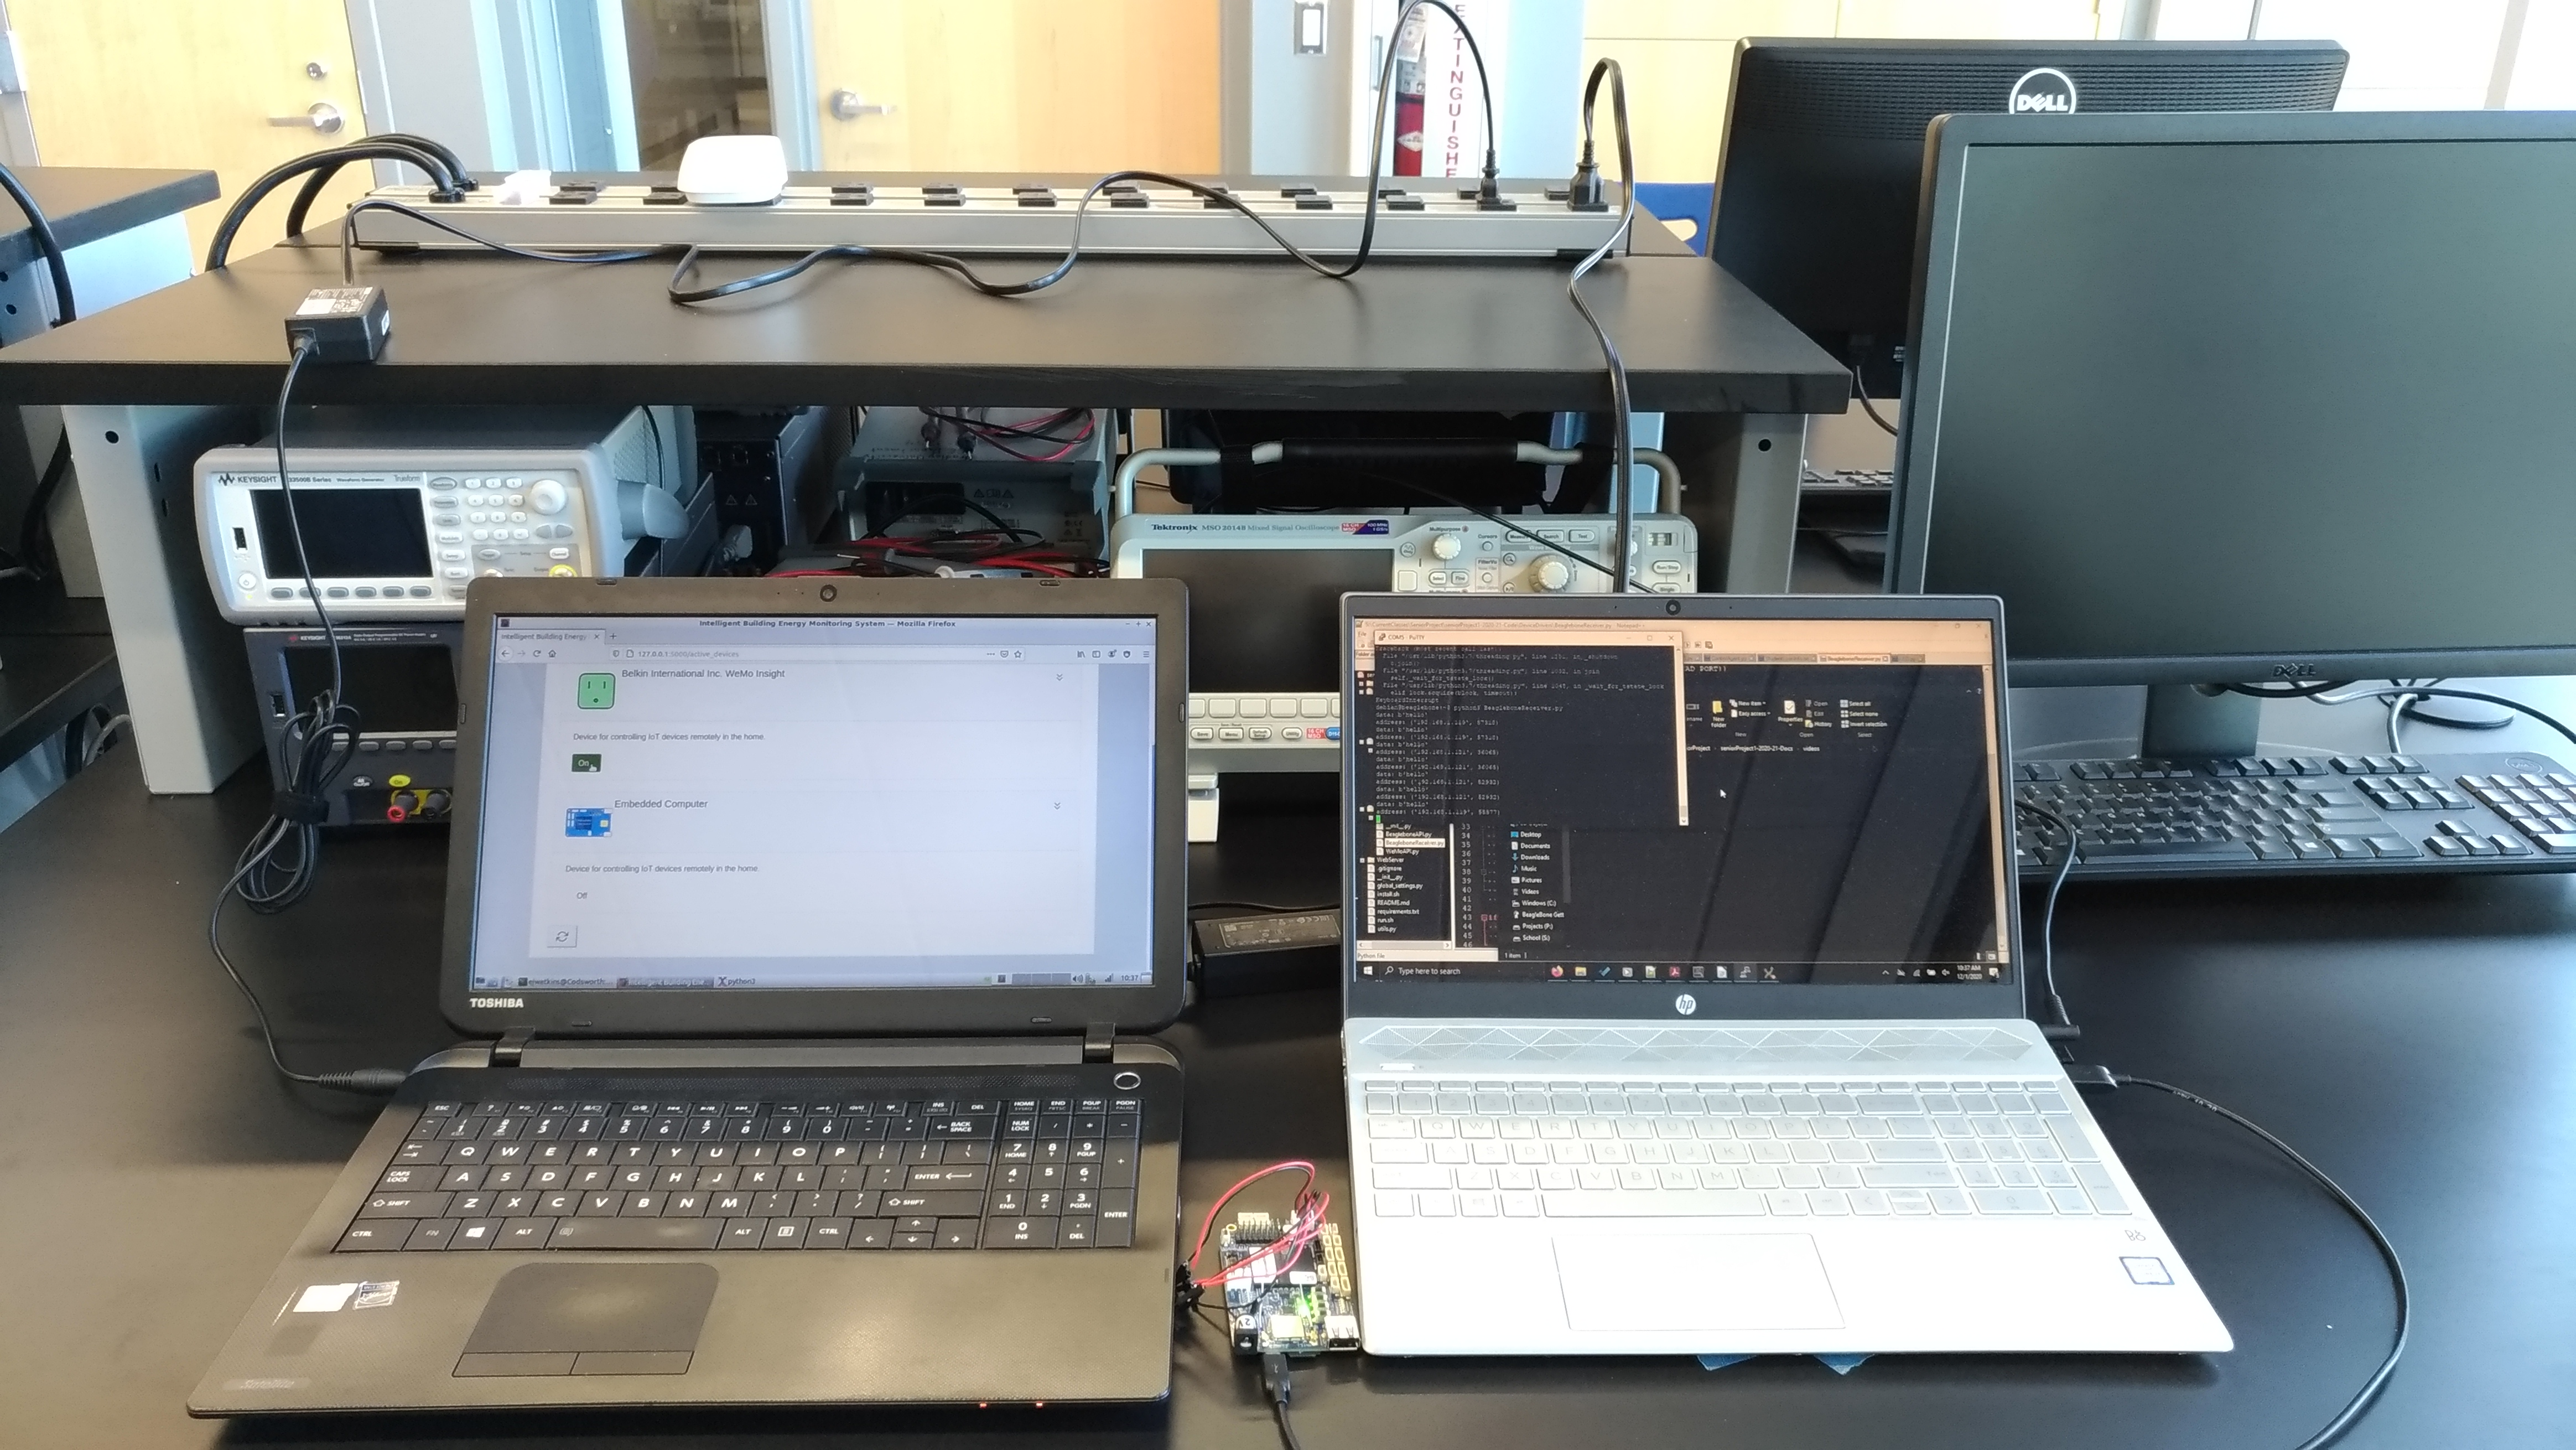
\includegraphics[scale=0.09]{figs/experimentalLabSetup.jpg}
    \caption{Actual lab setup for testing WeMo Insight Switch and embedded computer}
    \label{fig:expLabSetup}
\end{figure}

\subsection{Experimental Activities} \label{sec:expresults}
Up to this point, work has been completed on the web user interface which was developed with the Bootstrap CSS framework and the JQuery Javascript framework. The active device page in Figure~\ref{fig:activeDevicesPageScreenCap} displays the current controllable devices in the software. When a request is sent to the active devices URL, the discovery agent will ping all possible supported devices on the network and newly discovered devices will appear on the active devices page. Upon pressing the refresh button below the list of controllable devices, all buttons and icons will update with the current status obtained over the network. For example, the refresh button will cause the position of the slide switch shown to change depending on whether the WeMo switch is on or off. The top nav bar will link to other pages including the home page, applications page, notifications and settings page. However, only the active devices page has been implemented.

\begin{figure}
    \centering
    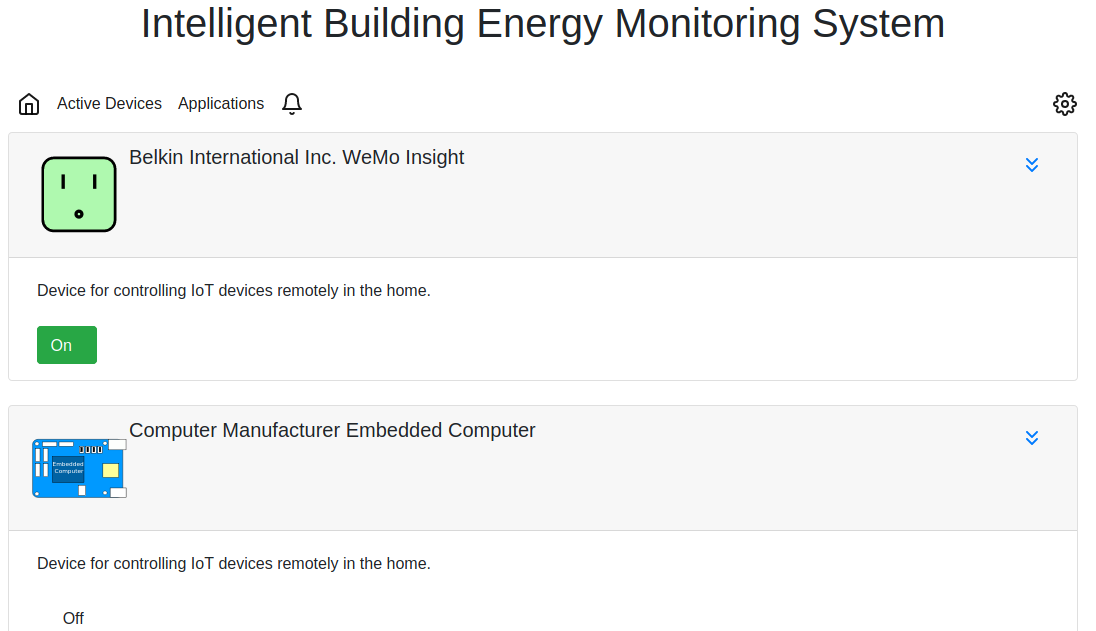
\includegraphics[scale=0.4]{figs/activeDevicesWithEmbeddedPicture.png}
    \caption{Screenshot of Web Server (Active Devices Page)}
    \label{fig:activeDevicesPageScreenCap}
\end{figure}

Figure~\ref{fig:powerPlotWeMoSwitch} shows a plot of the Wemo power usage using data we collected during lab hours.

\begin{figure}[H]
    \centering
    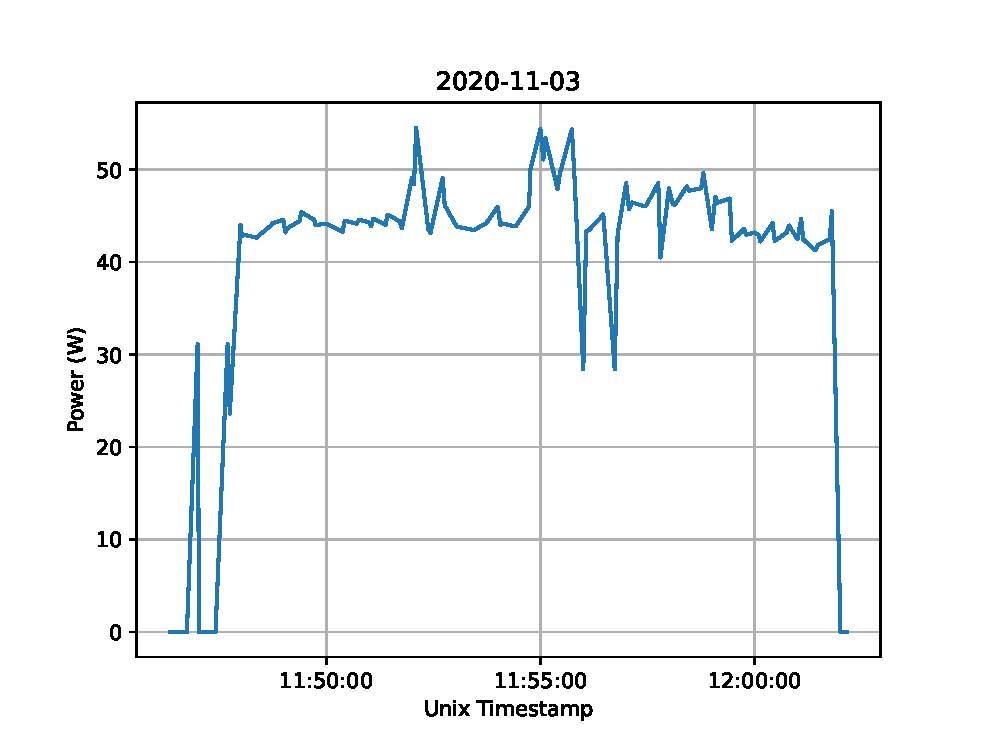
\includegraphics[scale=0.5]{figs/powerPlot2020-11-03.eps}
    \caption{Plot of WeMo Switch power usage 2020-11-03}
    \label{fig:powerPlotWeMoSwitch}
\end{figure}

\section{Parts List}
This project is mostly code-based, but we are physically implementing the WeMo Insight Switch and BeagleBone Blue embedded computer as well as some extra hardware. The following list is rather short, but comprehensive for our purposes.

\begin{itemize}
    \item WeMo Insight Smart Plug
    \item BeagleBone Blue
    \begin{itemize}
        \item Octavo OSD3358 Microprocessor
        \item Wifi/Bluetooth
        \item IMU/Barometer
        \item Power Regulation and state-of-charge LEDs for a 2-cell LiPo
        \item H-Bridges
        \item Connectors for 4 DC motors and 8 Servos
    \end{itemize}
    \item JST-ZH connector (for BeagleBone Blue Motor Connections)
    \item DC Motor
    \item ECE department laptop
    \item ECE department lab router
\end{itemize}

\begin{figure}[H]
    \centering
    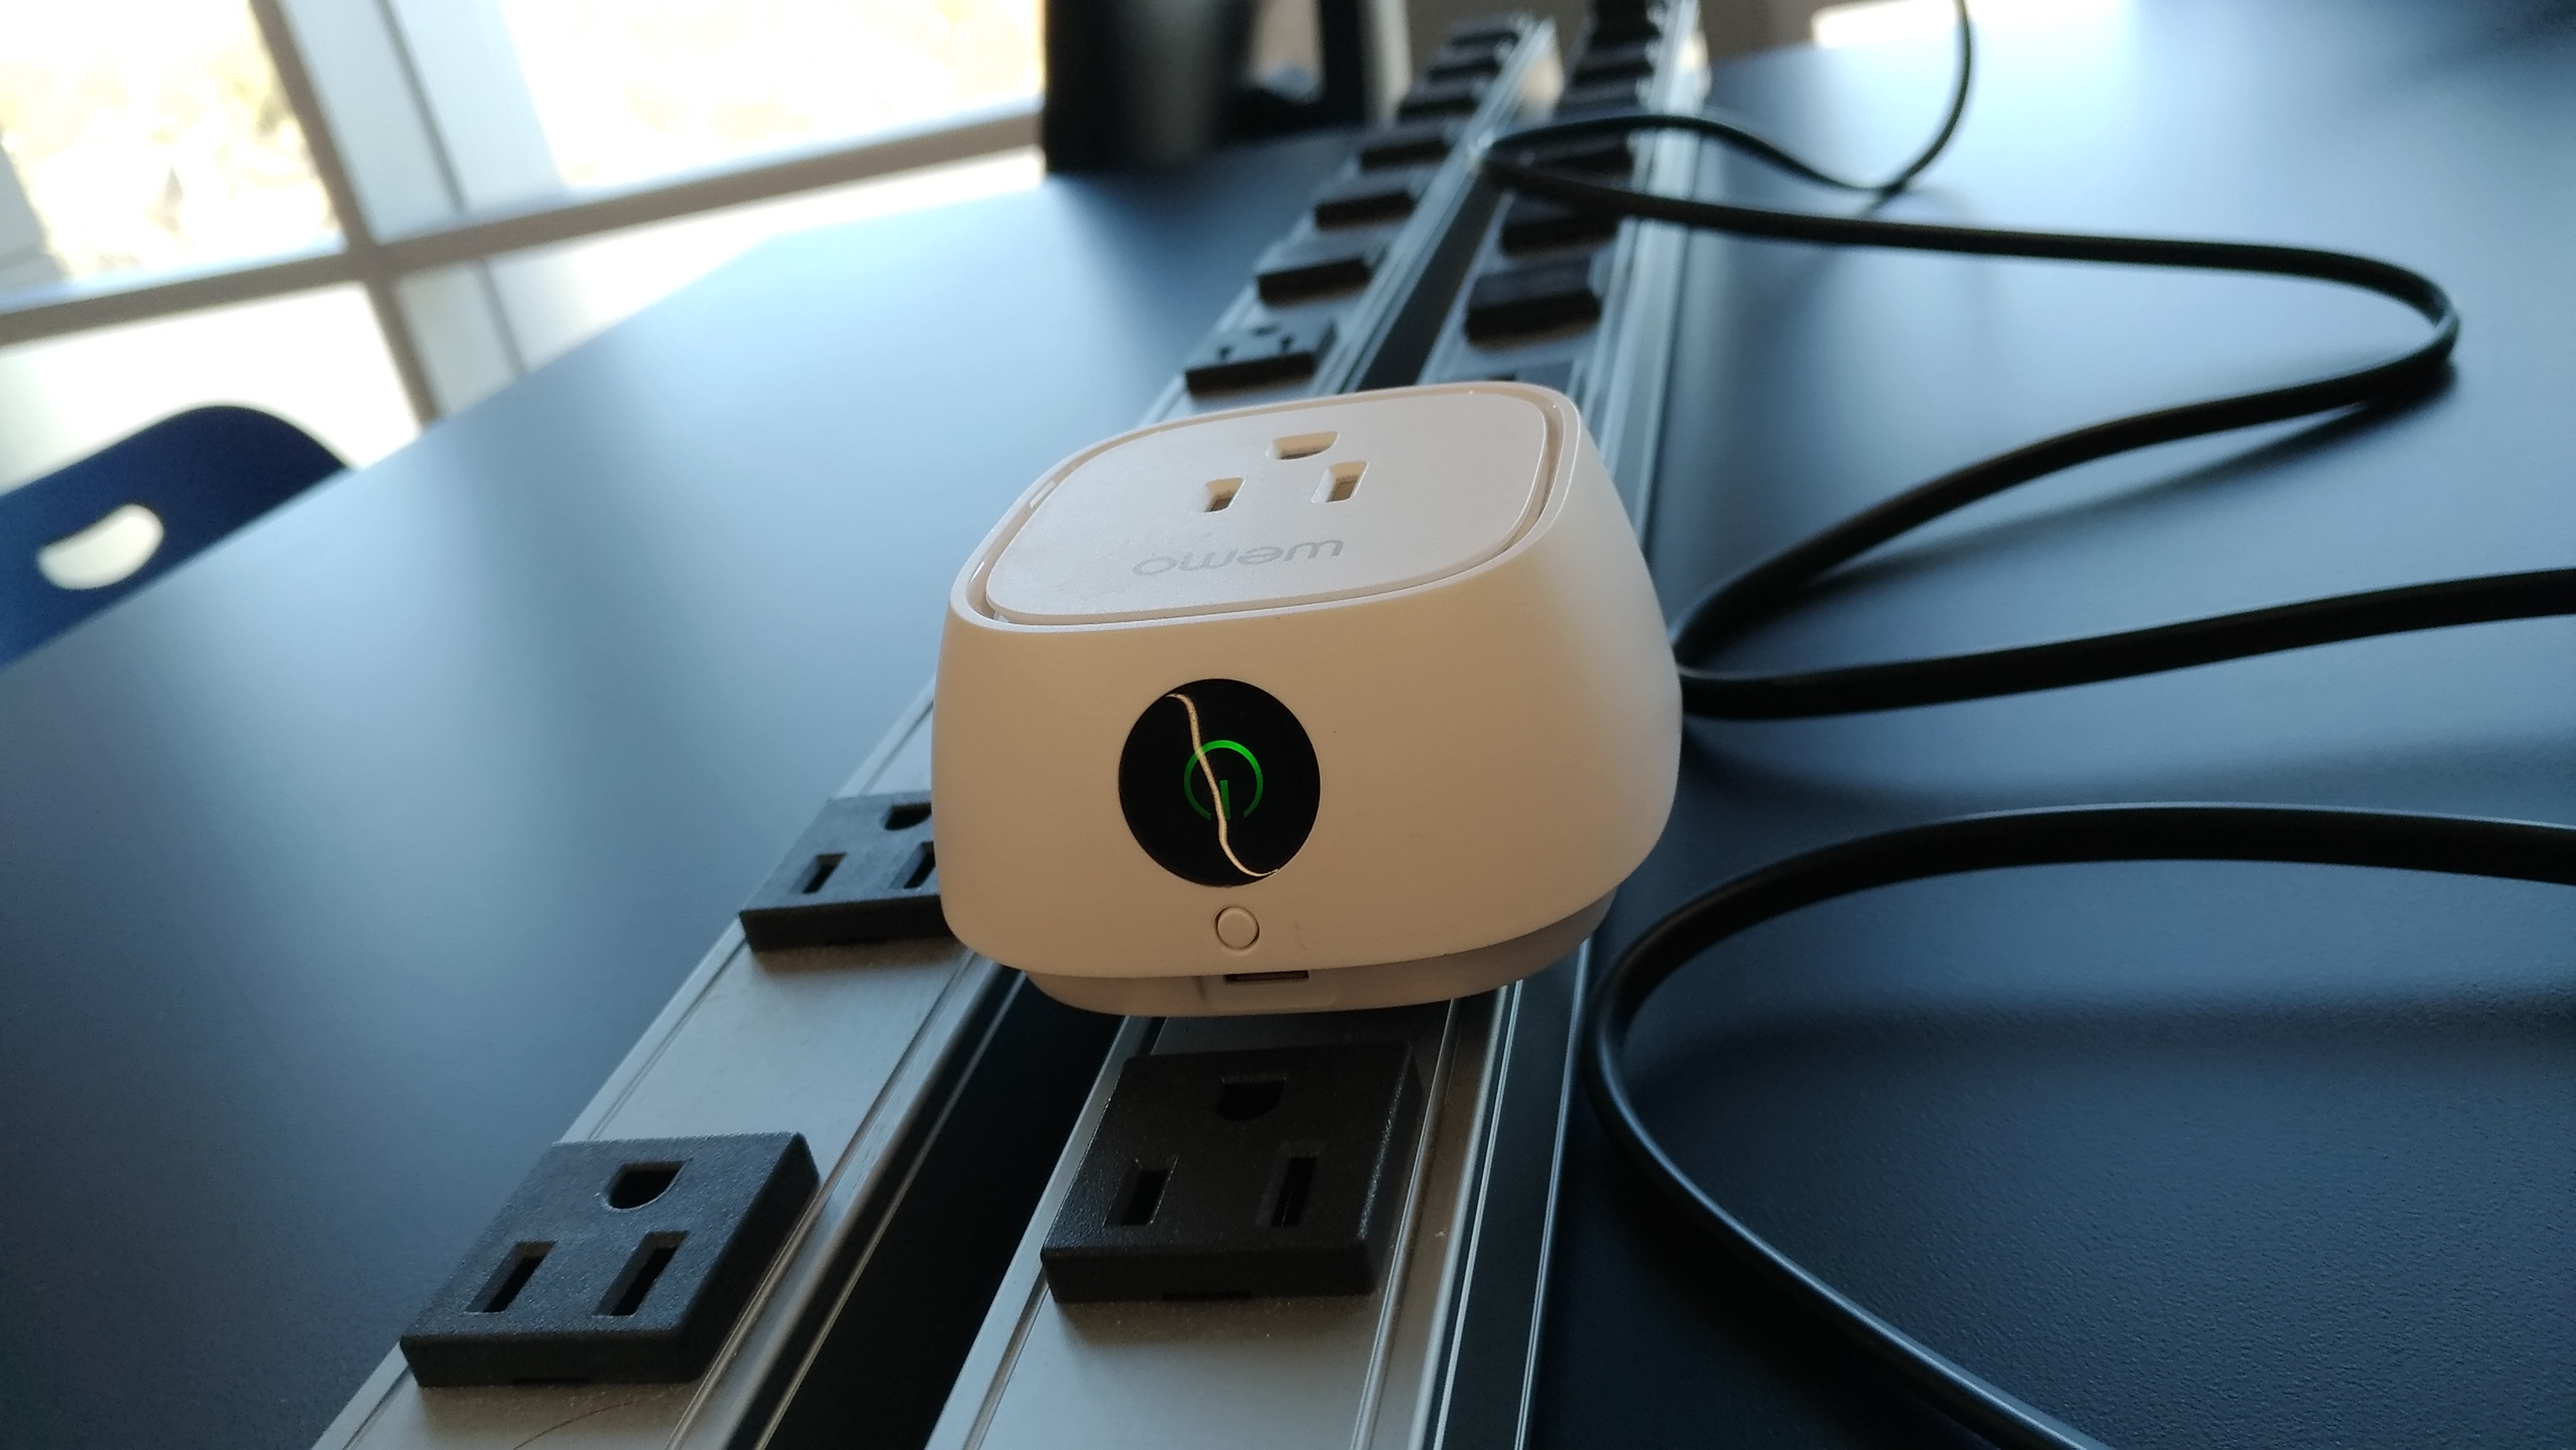
\includegraphics[scale=0.09]{figs/wemo.jpg}
    \caption{Photo of WeMo Insight Switch used in the lab}
    \label{fig:expLabSetup}
\end{figure}

\begin{figure}[H]
    \centering
    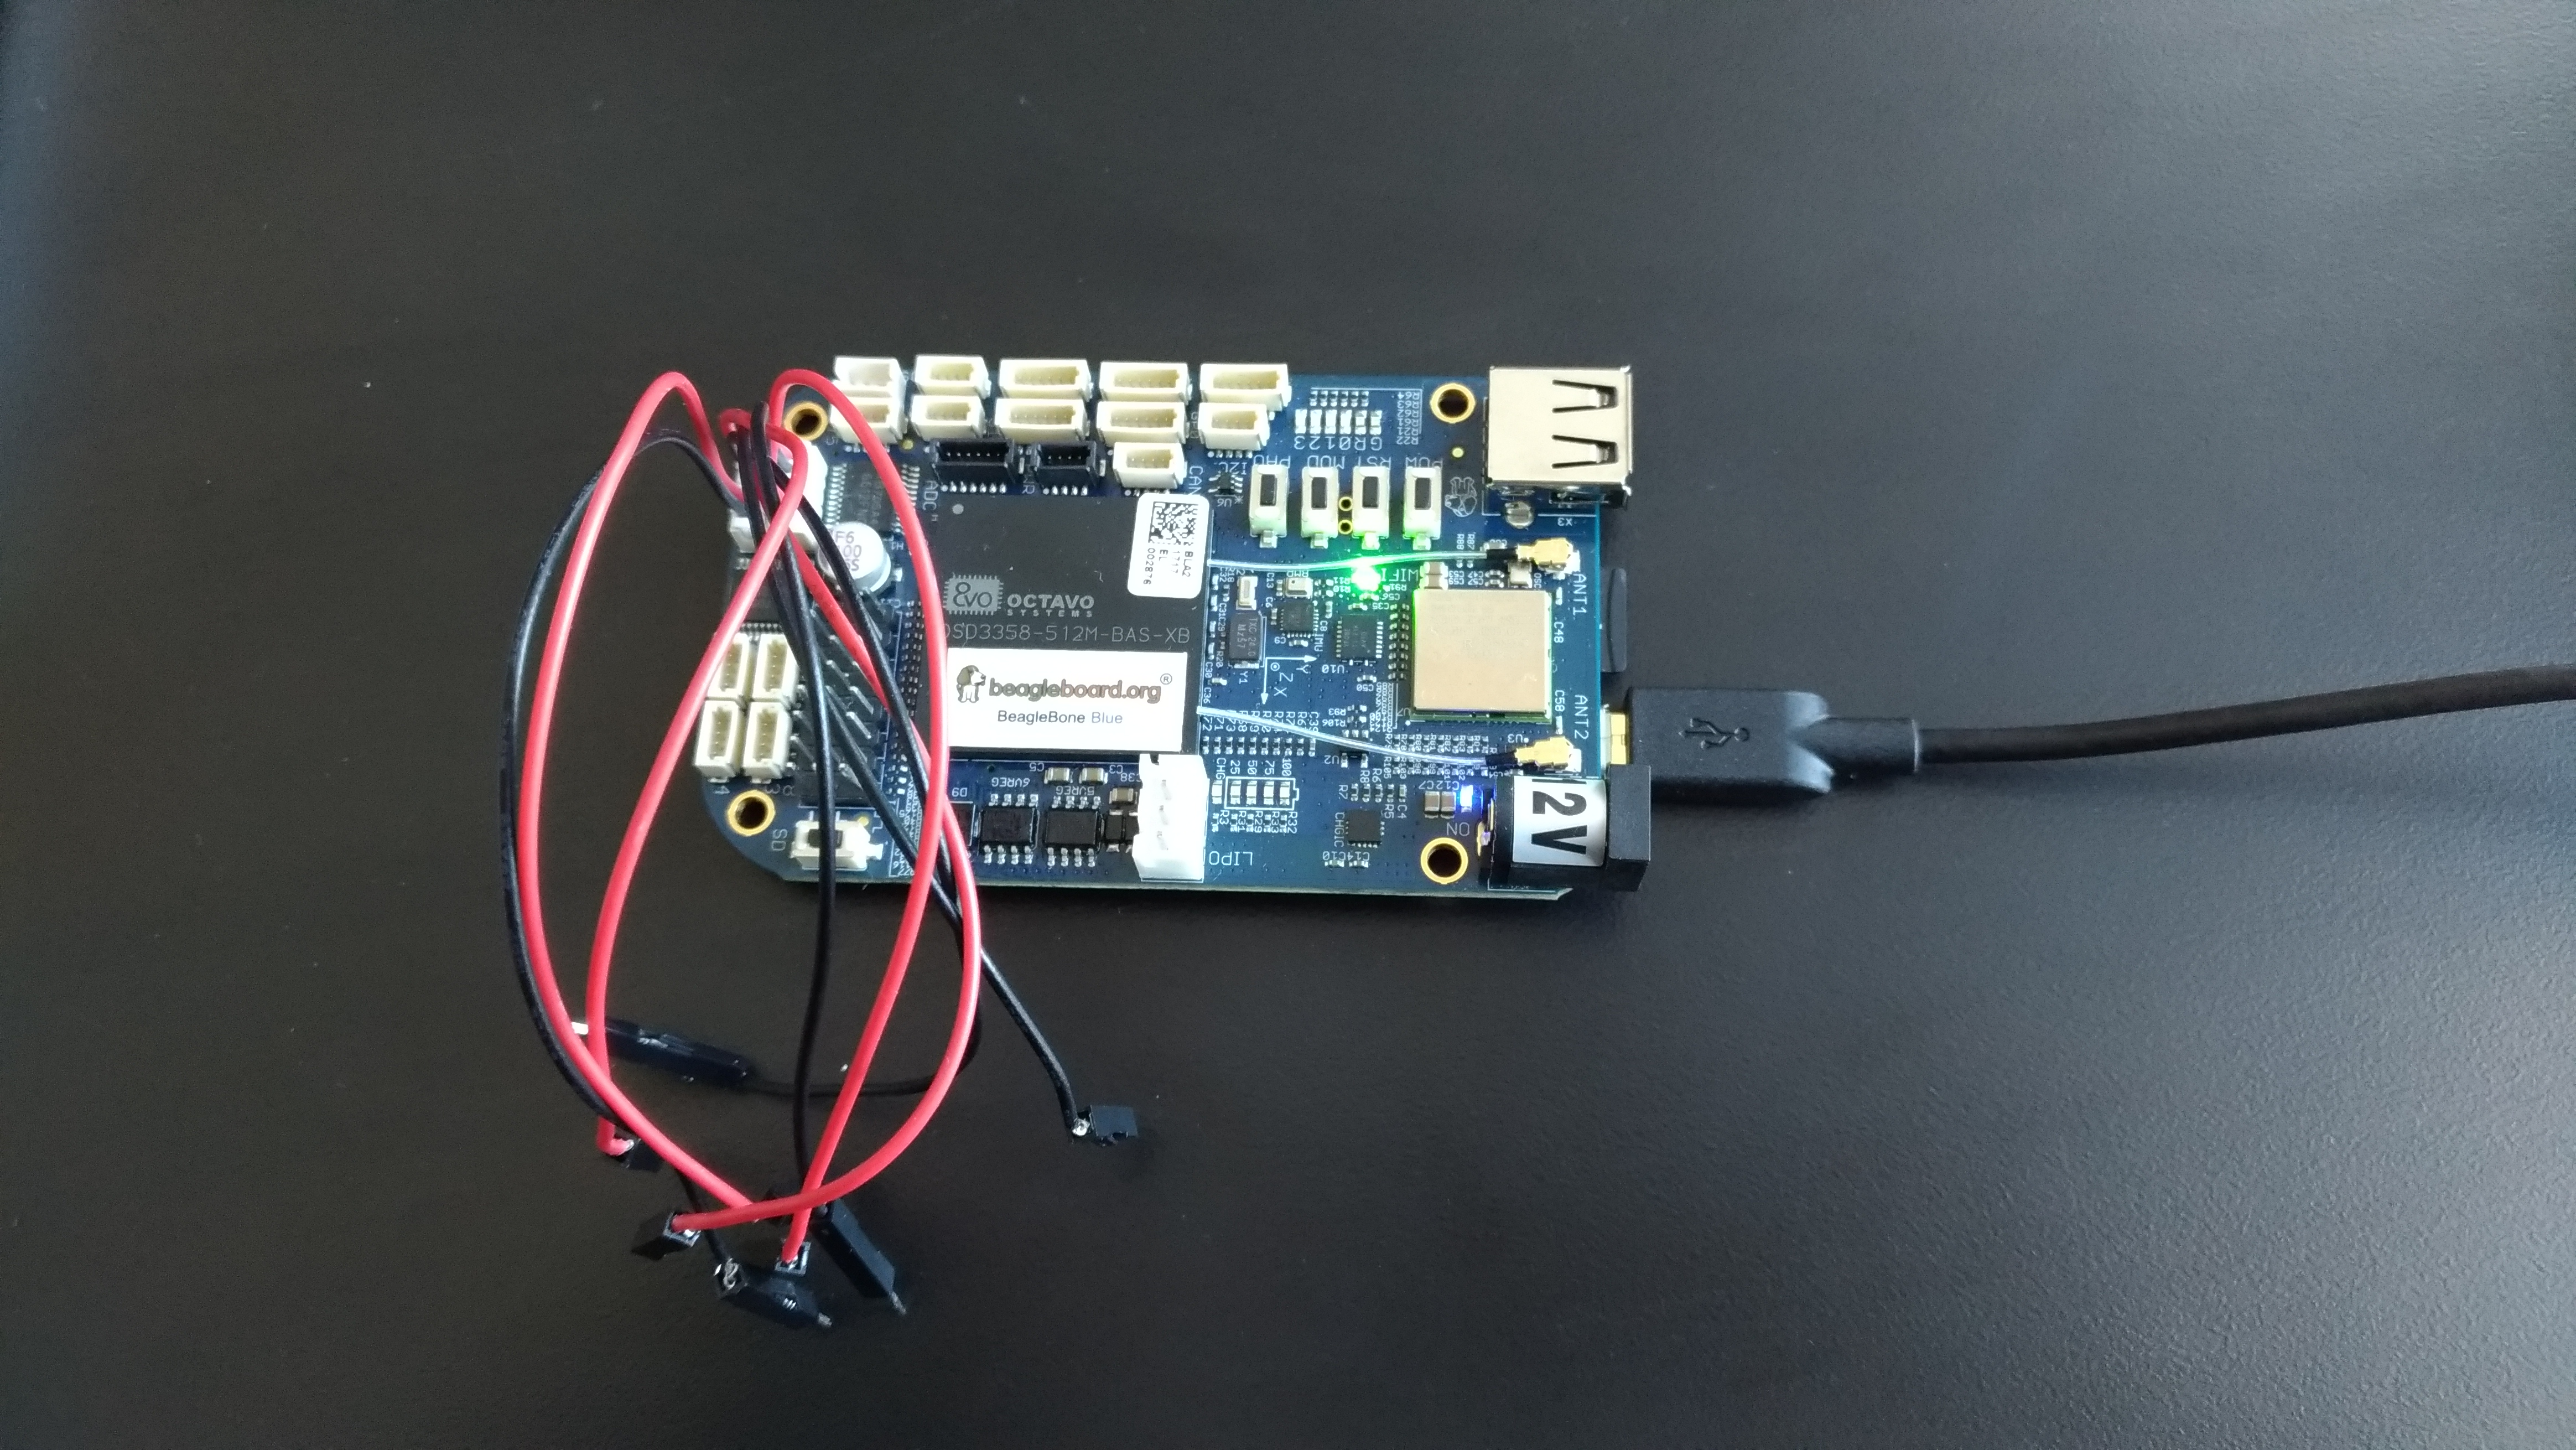
\includegraphics[scale=0.09]{figs/beagleBone.jpg}
    \caption{Photo of embedded computer (BeagleBone Blue) used in the lab}
    \label{fig:expLabSetup}
\end{figure}

\section{Timeline and Milestones} \label{sec:timeline}
During the first semester, Fall 2020, work will be done to further polish the WeMo Switch functionality like updating the status and obtaining the power usage. In order to further set up the platform, support for the Cassandra database will be added to store power usage and other device status information. Each entry in the database will be associated with a specific device and timestamp containing the current time and date. To visualize the data, a Matplotlib plot will be generated by reading data from a CSV file generated from the device status information. This plot will be displayed in the UI. DC motor support will be built through Beaglebone Blue connectivity over the TCP/IP bulding network. User login and management will be added to give users a more personalized experience in the platform. In the second semester, Spring 2021, algorithms will be developed to simulate and control both a microgrid and HVAC system along with integration in the platform. Lastly, as a final touch weather service support will be added along with notifications if time allows.

\begin{sidewaysfigure}
\begin{ganttchart}[hgrid,vgrid,x unit=.8cm, y unit title=.5cm,y unit chart=.8cm,milestone label font=\tiny,bar label font=\tiny, group label font=\small,bar/.append style={fill=green},bar incomplete/.append style={fill=red}]{1}{16}
\gantttitle{Fall 2020}{16}\\
\gantttitle{Sep}{4}
\gantttitle{Oct}{4}
\gantttitle{Nov}{4}
\gantttitle{Dec}{4}\\
\ganttgroup[progress = 100,group progress label font = \tiny,progress label text={$\displaystyle#1\%$},group progress label anchor = east]{WeMo Functionality}{3}{5} \\
\ganttbar[progress = 100,progress label text={$\displaystyle#1\%$},bar progress label font = \tiny,bar progress label anchor = east]{Refresh Status on Web Server}{3}{5}\\
\ganttbar[progress = 100,bar progress label font = \tiny,progress label text={$\displaystyle#1\%$},bar progress label anchor = east]{Record Power Usage}{3}{5}\\
\ganttgroup[progress = 67,group progress label font = \tiny,progress label text={$\displaystyle#1\%$},group progress label anchor = east]{Data Logging Feature}{5}{10}\\
\ganttbar[progress = 80,bar progress label font = \tiny,progress label text={$\displaystyle#1\%$},bar progress label anchor = east]{Support for Cassandra database}{5}{9}\\
\ganttbar[progress = 0,bar progress label font = \tiny,progress label text={$\displaystyle#1\%$},bar progress label anchor = east]{Matplotlib Plot in UI}{10}{10}\\

\ganttgroup[progress = 55,group progress label font = \tiny,progress label text={$\displaystyle#1\%$},group progress label anchor = east]{BeagleBone Functionality}{7}{14}\\
\ganttbar[progress = 90,bar progress label font = \tiny,progress label text={$\displaystyle#1\%$},bar progress label anchor = east]{Communication with BEMS}{7}{11}\\
\ganttbar[progress = 0,bar progress label font = \tiny,progress label text={$\displaystyle#1\%$},bar progress label anchor = east]{PWM Motor Control}{12}{13}\\
\ganttbar[progress = 0,bar progress label font = \tiny,progress label text={$\displaystyle#1\%$},bar progress label anchor = east]{Record Power Usage}{14}{14}\\
\end{ganttchart}
\caption{Gantt chart for Fall 2020}
\label{gantt1}
\end{sidewaysfigure}

%change this to the correct format and make our schedule
%\begin{landscape}
\begin{sidewaysfigure}
%\begin{figure}
%\centering
\begin{ganttchart}[hgrid,vgrid,x unit=.8cm, y unit title=.5cm,y unit chart=.8cm,milestone label font=\tiny,bar label font=\tiny, group label font=\small,bar/.append style={fill=green},bar incomplete/.append style={fill=red}]{1}{18}
\gantttitle{Spring 2021}{18}\\
\gantttitle{Jan}{4}
\gantttitle{Feb}{4}
\gantttitle{Mar}{4}
\gantttitle{Apr}{4}
\gantttitle{May}{2}\\
\ganttgroup[progress = 0,group progress label font = \tiny,progress label text={$\displaystyle#1\%$}, group progress label anchor = east]{Simscape Microgrid}{3}{8}\\
\ganttbar[progress = 0,bar progress label font = \tiny,progress label text={$\displaystyle#1\%$},group progress label anchor = east]{Setup Simscape Microgrid}{3}{5}\\
\ganttbar[progress = 0,bar progress label font = \tiny,progress label text={$\displaystyle#1\%$},group progress label anchor = east]{Get Power Meter Data}{6}{8}\\
\ganttgroup[progress = 0,group progress label font = \tiny,progress label text={$\displaystyle#1\%$},group progress label anchor = east]{HVAC Control}{9}{14} \\
\ganttbar[progress = 0,bar progress label font = \tiny,progress label text={$\displaystyle#1\%$},bar progress label anchor = east]{Create HVAC system in Simscape}{9}{11} \\
\ganttbar[progress = 0,bar progress label font = \tiny,progress label text={$\displaystyle#1\%$},bar progress label anchor = east]{Implement LQR Algorithm for HVAC Control}{12}{14} \\
%\ganttmilestone[progress = 0,milestone progress label font = \tiny,milestone progress label anchor = east]{Finalize Functionality}{5} \ganttnewline
\ganttgroup[progress = 0,group progress label font = \tiny,progress label text={$\displaystyle#1\%$},group progress label anchor = east]{Weather Service Update}{15}{16}\\
\ganttbar[progress = 0,bar progress label font = \tiny,progress label text={$\displaystyle#1\%$},group progress label anchor = east]{Receive Weather Data}{15}{15}\\
\ganttbar[progress = 0,bar progress label font = \tiny,progress label text={$\displaystyle#1\%$},group progress label anchor = east]{Display Notification}{16}{16}
\end{ganttchart}
\caption{Gantt Chart for Spring 2021}
\label{fig:gantt2}
%\end{figure}
\end{sidewaysfigure}
%\end{landscape}

\clearpage
\bibliographystyle{IEEEtran}
\bibliography{bib/references.bib}

\end{document} 